\documentclass[11pt]{article}

\usepackage{CMPSC465}
\usepackage{enumitem}
\usepackage{algpseudocode}
\usepackage{tikz}

\def\title{Assignment 04}

\def\defeq{\mathrel{\mathop:}=}
%\usepackage{algpseudocode}
%\usepackage{algorithm}
\usepackage[ruled,noline]{algorithm2e}
%\usepackage{amsthm}
\newcommand\nonl{%
  \renewcommand{\nl}{\let\nl\oldnl}}% Remove line number for one line
  
\newcommand{\aaa}[1]{\hspace{0.65cm}\parbox[t]{15.3cm}{#1}}
\newcommand{\aab}[1]{\hspace{1.15cm}\parbox[t]{15.0cm}{#1}}
\newcommand{\aac}[1]{\hspace{1.65cm}\parbox[t]{15.0cm}{#1}}
\newcommand{\aad}[1]{\hspace{2.15cm}\parbox[t]{15.0cm}{#1}}
\newcommand{\aaA}[2]{\hspace{0.5cm} {\tikz[overlay] \draw (0.1, -0.1) -- (0.1, #1 * -1.5em + 0.6em);} \parbox[t]{15.0cm}{#2}}
\newcommand{\aaB}[2]{\hspace{1.0cm} {\tikz[overlay] \draw (0.1, -0.1) -- (0.1, #1 * -1.5em + 0.6em);} \parbox[t]{15.0cm}{#2}}
\newcommand{\aaC}[2]{\hspace{1.5cm} {\tikz[overlay] \draw (0.1, -0.1) -- (0.1, #1 * -1.5em + 0.6em);} \parbox[t]{15.0cm}{#2}}
\newcommand{\aaD}[2]{\hspace{2.0cm} {\tikz[overlay] \draw (0.1, -0.1) -- (0.1, #1 * -1.5em + 0.6em);} \parbox[t]{15.0cm}{#2}}
\newcommand{\xxx}{\par\vspace{0.1cm}}

\begin{document}
\maketitle

\section*{Due: Friday 11:59 am, Feb.\ 11, 2022}

\paragraph*{Instructions:}

You may work in groups of up to three people to solve the homework.
You must write your own solutions and explicitly acknowledge everyone whom 
you have worked with or who has given you any significant ideas about your solutions. 
You may also use books or online resources to help solve homework problems.  
All consulted references must be acknowledged. The acknowledgements need to be made by answering Problem~1 below.

You are encouraged to solve the problem sets on your own using only the textbook and lecture notes as a reference. This will give you the best chance of doing well on the exams. Relying too much on the help of group members or on online resources will hinder your performance on the exams.

Submissions being late in 2 hours will be accepted with a 20\% penalty. Submissions late more than 2 hours will receive 0. There will be no exceptions to this policy, as we post the solutions soon after the deadline. 

For the full policy on assignments, please consult the syllabus.

\paragraph*{Formatting:} Start a new page for each problem.

\paragraph*{Describing an Algorithm:} Please make sure you use plain wording to explain your algorithm. It is always a good practice to start with a summary of the high-level idea of your algorithm to ease graders understand your solution quickly. Then, explain your algorithm, using plain wording and including enough details.

The use of pseudo-code is optional, and it is your decision. No matter you use it or not, above description in words is always required. The pseudo-code has its own advantage in explaining structured (i.e., if-else, for-loop, recursive functions, etc) algorithms and in putting details in the right place. If you think pseudo-code better explains your algorithm, and/or helps graders understand your solution, and/or contains more details not included in the plain-wording description, then use pseudo-code. If you think everything is already clearly explained in the description with words, then you don't need to include pseudo-code. An algorithm that is only written in pseudo-code (i.e., missing above plain-wording description) is not acceptable, as it is extremely hard to read just pseudo-code without any explanation.

Here is a general situation that may help you decide whether to use pseudo-code or not. An algorithm could be ``designed from scratch'', i.e., you will need to come up with the step-by-step procedure. This usually involves in implementing a function with clear input and output. In this case, including pseudo-code usually helps. All algorithm we've seen so far (e.g., merge-two-sorted-arrays, merge-sort, etc) falls in this category. Second, an algorithm could also be ''transformed into another algorithm'', i.e., you use an existing algorithm to solve this problem. In this case you usually don't need to include pseudo-code but to describe how to transform one problem into the other. We will see such examples soon.

\clearpage\newpage

\begin{qunlist}
\setcounter{sparectr}{-1}

\q{0}{Acknowledgements. }
	The assignment will receive a 0 if this question is not answered.
\begin{enumerate}
	\item If you worked in a group, list the members of the group. Otherwise, write ``I did not work in a group.''
	\item If you received significant ideas about your solutions from anyone not in your group, list their names here. Otherwise, write ``I did not consult  anyone except my group members''.
	\item List any resources besides the course material that you consulted in order to solve the material. If you did not consult anything, write ``I did not consult any non-class materials.''
\end{enumerate}

% Bucky
\q{15}{}
In class, we learned the following property about duality: point $p$ is on line $l$ if and only if point $l^*$ is on line $p^*$.
\begin{enumerate}
    \item Using the property above, prove the following properties:
    \begin{enumerate}
        \item If $n$ points $p_1, ..., p_n$ are on a common line $l$, then $p_1^*, p_2^*, ..., p_n^*$ intersect at a common point $l^*$.
        \item If $n$ lines $l_1, ..., l_n$ intersect at a common point $p$, then $l_1^*, l_2^*, ..., l_n^*$ are on a common line $p^*$.
    \end{enumerate}
    \item If we have a line segment $s$ connecting two points $p_1$ and $p_2$, describe a region $s^*$ corresponding to the dual of $s$ in terms of $p_1^*$ and $p_2^*$. (No rigorous proof is needed.)
    \item If a line $l$ intersects the line segment $s$, prove that $l^*$ is in the region $s^*$.
\end{enumerate}

%Bucky
\q{15}{} We are given a graph $G = (V, E)$; $G$ could be a directed graph or undirected graph. Let $M$ be the adjacency matrix of $G$. Let $n$ be the number of vertices so that the matrix $M$ is $n \times n$ matrix. For any matrix $A$, let us denote the element of $i$-th row and $j$-th column of the matrix $A$ by $A[i, j]$.
\begin{enumerate}
    \item Consider the square of the adjacency matrix $M$. For all $i$ and $j$, show that $M^2[i, j]$ is the number of different paths of length $2$ from the $i$-th vertex to the $j$-th vertex. It should be explained or proved as clearly as possible.
    \item For any positive integer $k$, show that $M^k[i, j]$ is the number of different paths of length $k$  from the $i$-th vertex to the $j$-th vertex. You may use induction on $k$ to prove it.
    \item Assume that we are given a positive integer $k$. Design an algorithm to find the number of different paths of length $k$ from the $i$-th vertex to $j$-th vertex for all pairs of $(i,j)$. The time complexity of your algorithm should be $O(n^3 \log k)$. You can get partial credits if you design an algorithm of $O(n^3 k)$.
\end{enumerate}

\q{10}{}
You are given a grid of size $n\times m$ and within that grid there is a
horizontal rod~(arbitrary width but height of 1). You aim is to locate it. The only thing you can use to find the
location of the rod is make queries of the form IsPresent~$(x_1,y_1,x_2,y_2)$
where $x_1 \leq x_2 , y_1 \leq y_2$. This returns True if part of the rod is
present in the grid from $(x_1,y_1)$ to $(x_2,y_2)$ and False if not. See figures below.  Design
an algorithm which uses queries $O(\log(n + m))$ times to find the location of the rod, i.e., the leftmost coordinates and rightmost coordinates.
\emph{Hint: consider using binary search in your algorithm.}

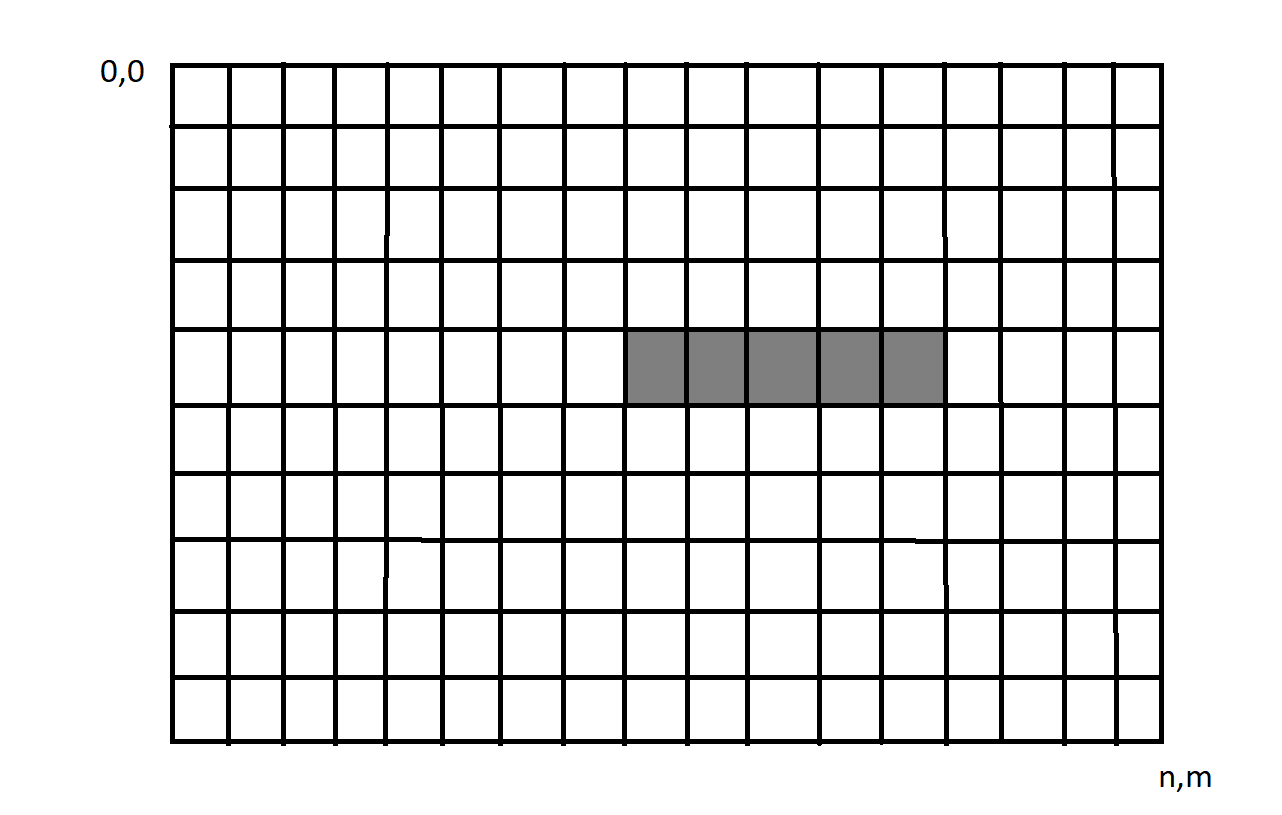
\includegraphics[width=\textwidth]{rod.png}
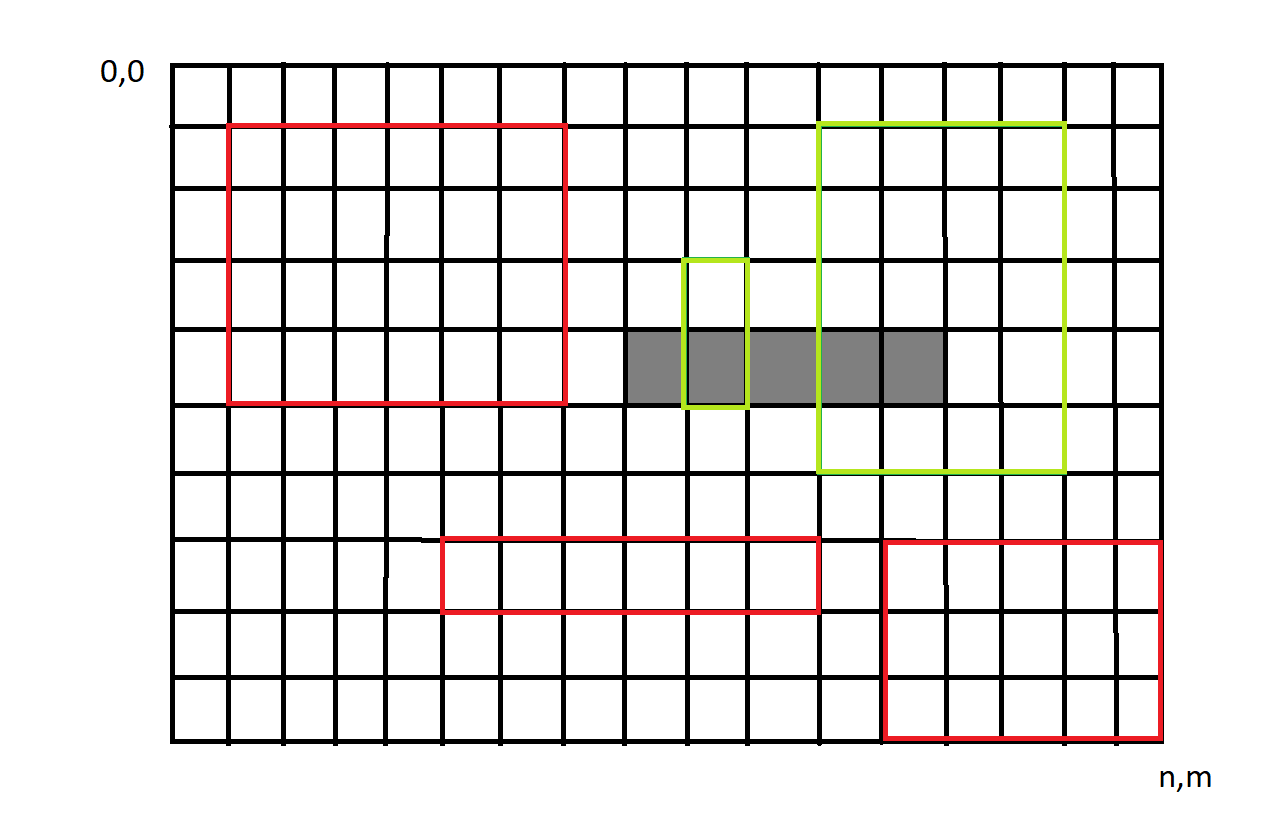
\includegraphics[width=\textwidth]{query.png}



\end{qunlist}
\end{document}
